Contar con una gran cantidad de datos en cualquier problema de detecci\'{o}n de anomal\'{i}as es lo que permite generar modelos m\'{a}s precisos, debido a que nunca se sabe qu\'{e} caracter\'{i}sticas pueden dar indicio de una anomal\'{i}a, contar con m\'{u}ltiples tipos de datos es lo que permite ir m\'{a}s all\'{a} de una mera detecci\'{o}n de anomal\'{i}as puntuales y ser capaz de identificar anomal\'{i}as contextuales o colectivas m\'{a}s sofisticadas. Sin embargo la obtenci\'{o}n de estos datos no siempre es una tarea sencilla, por lo que muchas veces se debe encontrar una manera de generar los mismos.

\vspace{5mm} %5mm vertical space

En este cap\'{i}tulo se detallar\'{a} el m\'{e}todo de recolecci\'{o}n de datos que se realizar\'{a} para la presente investigaci\'{o}n y las diferentes t\'{e}cnicas de an\'{a}lisis de datos que se aplicar\'{a}.

\section{Captura de datos}

Actualmente existen varios enfoques para acceder a la información del conductor y del vehículo. En el primer enfoque, un conjunto de sensores y hardware adicional se implementan previamente en el veh\'{i}culo, por ejemplo, cajas telemáticas (cajas negras provistas por compañías de seguros de automóviles), adaptadores de diagnóstico a bordo (OBD-II) enchufados en el controlador del vehículo red de área (CAN) (\cite{30}, \cite{31}), la información registrada por estos dispositivos se puede recuperar o enviar a través de Internet. Sin embargo, esta estrategia requiere que los vehículos instalen dispositivos adicionales, lo que implica un mayor costo. Para superar estos inconvenientes, existe un enfoque alternativo el cual es usar teléfonos inteligentes para recopilar datos a través de un conjunto de sensores integrados, tales como sensores inerciales (acelerómetros y giroscopios), sistemas de posicionamiento global (GPS), magnetómetros, micrófonos, sensores de imagen (cámaras), sensores de luz , sensores de proximidad, sensores de dirección (brújula), entre otros.

\vspace{5mm} %5mm vertical space

Para el presente trabajo de grado se eligi\'{o} el uso de tel\'{e}fonos inteligentes para acceder a la informaci\'{o}n del tipo de conducci\'{o}n, por las razones que se presentaron anteriormente, con este enfoque se desarroll\'{o} una aplicaci\'{o}n m\'{o}vil basada en Android para recopilar datos de los sensores: aceler\'{o}metro y giroscopio, en intervalos de 1 segundo, los cuales en una primera instancia ser\'{a}n almacenados de manera interna en el dispositivo m\'{o}vil. (Ver Figura \ref{fig:captura})


\vspace{5mm} %5mm vertical space

\begin{figure}[h!]
  \begin{center}	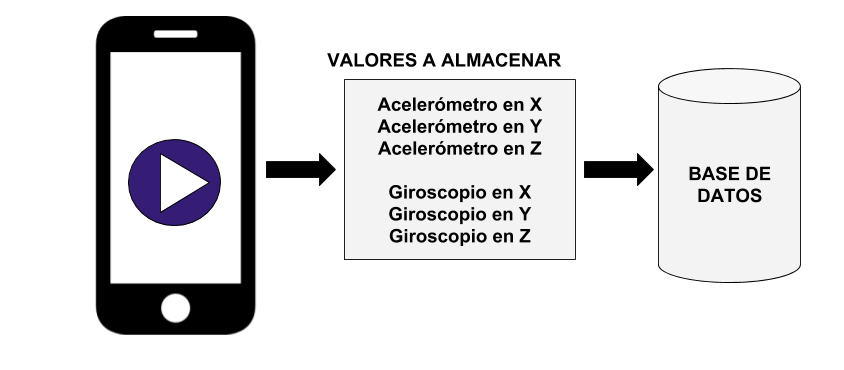
\includegraphics[width=0.95\textwidth]{imagenes/captura}
  \caption{Recolecci\'{o}n de datos, con intervalo de un segundo.}
  \label{fig:captura}
  \end{center}
\end{figure}


\vspace{5mm} %5mm vertical space

Para la captura de datos se us\'{o} un soporte para celular de parabrisas como se ve en la Figura \ref{fig:soporte}; se realiz\'{o} la captura en dos posiciones distintas (vertical y horizontal).
\vspace{5mm} %5mm vertical space

\begin{figure}[h!]
  \begin{center}	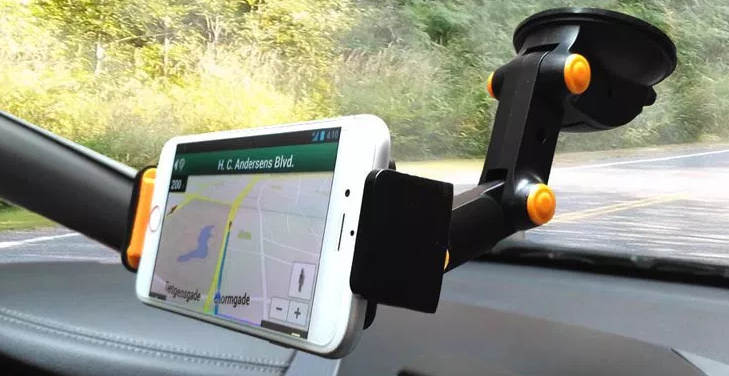
\includegraphics[width=0.65\textwidth]{imagenes/soporte}
  \caption{Soporte para celular de parabrisas, posici\'{o}n horizontal.}
  \label{fig:soporte}
  \end{center}
\end{figure}

Cada captura, independientemente de la posici\'{o}n en la que se realiz\'{o}, di\'{o} como resultado un conjunto de datos (dataset), donde por cada tiempo T (1 seg.) se tiene seis variables: aceler\'{o}metro en X (acc x), aceler\'{o}metro en Y (acc y), aceler\'{o}metro en Z (acc z), giroscopio en X (gyr x), giroscopio en Y (gyr y) y giroscopio en Z (gyr z). En la Figura \ref{fig:dataset} se aprecia un fragmento del conjunto de datos que se obtuvo en una captura.

\begin{figure}[h!]
  \begin{center}	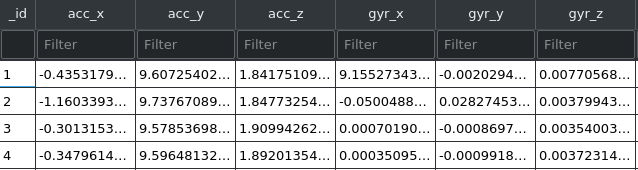
\includegraphics[width=0.85\textwidth]{imagenes/dataset}
  \caption{Fragmento del conjunto de datos obtenido.}
  \label{fig:dataset}
  \end{center}
\end{figure}

\section{An\'{a}lisis de los datos}

Como se indic\'{o} en la anterior secci\'{o}n, se realiz\'{o} la captura de datos del manejo de un usuario (conductor), de forma vertical y horizontal, a continuaci\'{o}n se analizar\'{a} las diferencias entre ellos.

\vspace{5mm} %5mm vertical space

En la Figura \ref{fig:verHor} se muestra fragmentos de las capturas obtenidas por el dispositivo m\'{o}vil del manejo de un mismo usuario desde diferentes posiciones.

\begin{figure}
        \centering
        \begin{subfigure}[h]{0.47\textwidth} 
            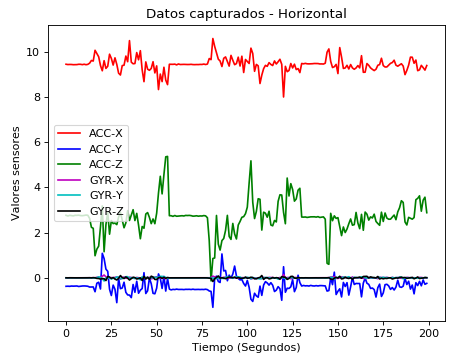
\includegraphics[width=\textwidth]{imagenes/horizontal}
            \caption{Captura de datos en horizontal}
            \label{fig:hor}
        \end{subfigure}       
        \begin{subfigure}[h]{0.47\textwidth} 
            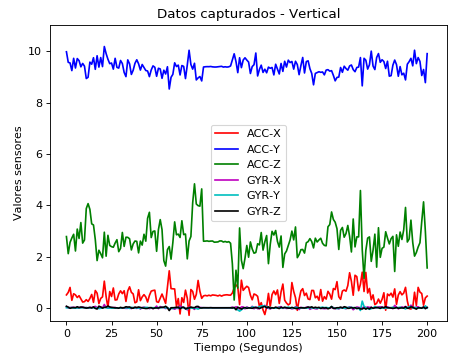
\includegraphics[width=\textwidth]{imagenes/vertical}
            \caption{Captura de datos en vertical}
            \label{fig:ver}
        \end{subfigure}
        \caption{Grafica de los sensores capturados en diferentes posiciones}
        		\label{fig:verHor}
    \end{figure}

\vspace{5mm} %5mm vertical space

Si bien los valores capturados, son muy similares entre s\'{i}, los datos que fueron capturados con el dispositivo m\'{o}vil en posici\'{o}n horizontal, presentan menos ruido, esto debido a que esta posici\'{o}n favorece la inercia del dispositivo cuando el veh\'{i}culo est\'{a} en movimiento, lo cual es una gran ventaja frente a los datos que fueron capturados de forma vertical, ya que estos fueron m\'{a}s suceptibles a sacudirse mientras el veh\'{i}culo se desplazaba haciendo que los valores capturados en esta posici\'{o}n presenten valores de movimiento no s\'{o}lo del veh\'{i}culo sino tambi\'{e}n del dispositivo m\'{o}vil, lo cual no es lo que se busca en el presente trabajo.

\vspace{5mm} %5mm vertical space

Por las razones presentadas en el anterior p\'{a}rrafo se decidi\'{o} trabajar con los datos capturados con el dispositivo m\'{o}vil en posici\'{o}n horizontal.

\vspace{5mm} %5mm vertical space

Para conseguir un an\'{a}lisis m\'{a}s profundo de los datos capturados durante la conducci\'{o}n de un veh\'{i}culo, a continuaci\'{o}n se presenta una tabla con los par\'{a}metros estad\'{i}sticos (Valor m\'{i}nimo, Valor m\'{a}ximo, Media, Mediana, Desviaci\'{o}n est\'{a}ndar) resultantes para cada columna de datos capturada (Tabla \ref{tab: est}).

%%%%%%%%%%
\begin{center}
\begin{table}[]
\begin{center}
\begin{tabular}{|l|l|l|l|l|l|l|}
\hline
 & \textbf{ACC-X} & \textbf{ACC-Y} & \textbf{ACC-Z} &  \textbf{GYR-X} & \textbf{GYR-Y} & \textbf{GYR-Z} \\ \hline
\textbf{Min} & -16.1556 & -11.5167 & -11.2487 & -3.0617 & -3.2679 & -4.7595 \\ \hline
\textbf{Max} & 15.5559 & 11.3349 & 15.2552 & 4.3997 & 2.3482 & 2.9745 \\ \hline
\textbf{Media} & 9.5361 & -0.7939 & -0.4447 & 0.0015 & 0.0003 &-0.0011 \\ \hline
\textbf{Mediana} & 9.7751 & -0.9049 & -0.4820 & -0.0001 & 6.1035e-05 & 6.1035e-05 \\ \hline
%\textbf{Moda} & 0, 9.7976 & 0, -0.8294 & 0, -0.997, -0.218 & 0, -0.000046 & 0, -0.000015 & 0, -0.00015 \\ \hline
\textbf{Des. est.} & 1.7220 & 1.3904 & 0.9007 & 0.0905 & 0.0857 & 0.1042 \\ \hline

\end{tabular}

\end{center}
\caption{Tabla de resultados estad\'{i}sticos del conjunto de datos.}
\label{tab: est}
\end{table}
\end{center}

\vspace{5mm} %5mm vertical space

Con la informaci\'{o}n proporcionada por la tabla ahora resulta m\'{a}s sencillo realizar un an\'{a}lisis del conjunto de datos, en primer lugar se evidencia que los valores obtenidos durante la captura, con el uso del dispositivo m\'{o}vil, se presentan entre rangos de valores muy distintos, se puede observar por ejemplo, que el valor del aceler\'{o}metro en X oscila entre los valores de -16 y 15 aproximadamente, mientras que los valores del giroscopio en X se encuentran entre -3 y 4, lo cual representa un problema debido a que \'{e}sta diferencia de rangos puede generar m\'{a}s peso en unos datos que en otros.

\vspace{5mm} %5mm vertical space

Para apreciar de una manera m\'{a}s gr\'{a}fica el problema expuesto con anterioridad a continuaci\'{o}n se presenta histogramas de las frecuencias de valores por cada tipo de par\'{a}metros que existe en el conjunto 
de datos. (Ver Figura \ref{fig:hist})

\begin{figure}[h!]
  \begin{center}	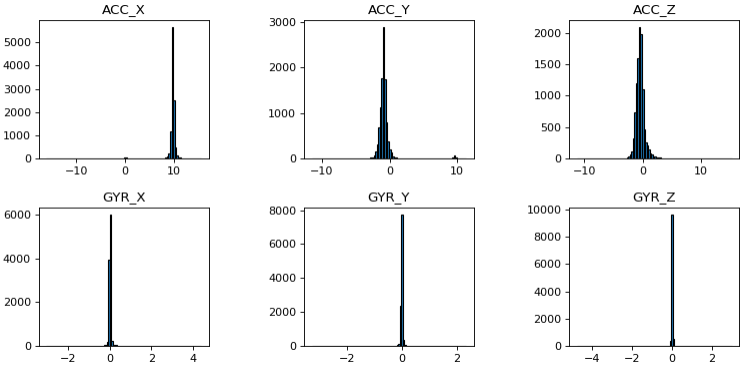
\includegraphics[width=0.97\textwidth]{imagenes/histogramaNormal}
  \caption{Histograma de frecuencias del conjunto de datos}
  \label{fig:hist}
  \end{center}
\end{figure}

Para solucionar este problema existe diversas t\'{e}cnicas, las cuales se abordar\'{a}n en la siguiente secci\'{o}n.

\subsection{Normalizaci\'{o}n}

La normalizaci\'{o}n de datos es un proceso o t\'{e}cnica para comprimir o extender los valores de una variable para que \'{e}sten en un rango definido, lo cual hace que muchos algoritmos de Aprendizaje Autom\'{a}tico funcionen mejor, sin embargo, una mala aplicaci\'{o}n de este proceso, o una elecci\'{o}n descuidada del m\'{e}todo de normalizaci\'{o}n puede arruinar los datos.

\vspace{5mm} %5mm vertical space

A continuaci\'{o}n se presenta algunos ejemplos de los m\'{e}todos de normalizaci\'{o}n m\'{a}s utilizados.

\subsubsection{Escalado de variables (Feature Scaling o MinMax Scaler)}

En este m\'{e}todo, cada entrada se normaliza entre unos l\'{i}mites definidos:

\begin{equation}
x_{normalizado} = \frac{x - x_{min}}{x_{max}-x_{min}}
\end{equation}

Presenta el problema de que comprime los datos de entrada entre unos límites fijos, que por lo general son 0 y 1. Esto quiere decir que si existe ruido, éste va a ser ampliado, lo que hace que este m\'{e}todo no sea adecuado para señales estables.

\subsubsection{Escalado est\'{a}ndar (Standard Scaler)}

Es un m\'{e}todo alternativo al escalado de variables, consiste en restar a cada dato la media de la variable y dividirlo por la desviaci\'{o}n t\'{i}pica.

\begin{equation}
x_{normalizado} = \frac{x - x_{media}}{x_{desvSt}}
\end{equation}

\'{E}ste m\'{e}todo si ser\'{i}a adecuado para normalizar se\~{n}ales estables, no obstante, tanto la media como la desviaci\'{o}n est\'{a}ndar son muy sensibles a valores an\'{o}malos. Una alternativa de soluci\'{o}n de esto ser\'{i}a la eliminaci\'{o}n de anomal\'{i}as antes de realizar la normalizaci\'{o}n.

\subsubsection{Escalado sobre el valor m\'{a}ximo}

El siguiente m\'{e}todo, presenta la idea de escalar los datos dividiendo \'{e}stos entre su m\'{a}ximo valor.

\subsubsection{Escalado robusto (Robust scaler)}

El escalado robusto consiste en eliminar la mediana y escala los datos de acuerdo con el rango de interquartil (IQR). Este m\'{e}todo es robusto para valores at\'{i}picos.

\vspace{5mm} %5mm vertical space

A continuaci\'{o}n se elaborar\'{a} un an\'{a}lisis para decidir que t\'{e}cnica de normalizaci\'{o}n es la m\'{a}s adecuada para escalar los par\'{a}metros de conducci\'{o}n capturados, en la Figura \ref{fig:datos_puros} se puede apreciar una fracci\'{o}n del conjunto de datos capturado, la cual es la base con la que se realizar\'{a} el an\'{a}lisis comparativo con los distintos tipos de normalizaci\'{o}n.

\begin{figure}[h!]
  \begin{center}	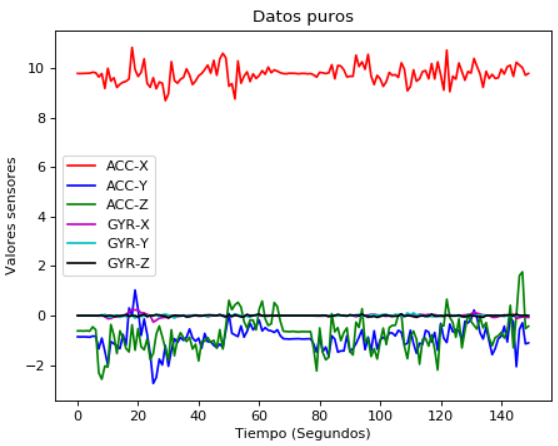
\includegraphics[width=0.5\textwidth]{imagenes/Cap3/datosPuros}
  \caption{Visualizaci\'{o}n de los par\'{a}metros de conducci\'{o}n capturados.}
  \label{fig:datos_puros}
  \end{center}
\end{figure}

\vspace{5mm} %5mm vertical space

El primer tipo de escalado que se realiz\'{o} sobre el conjunto de datos capturados fue el \textbf{escalado de variables}, el cual se realiz\'{o} entre los l\'{i}mites 0 y 1, los resultados obtenidos se muestran en la figura \ref{fig:min_max}, donde se puede apreciar que los valores del aceler\'{o}metro, en sus tres ejes, no se veen deformados despu\'{e}s de haber sido escalados con \'{e}sta t\'{e}cnica y los valores del giroscopio, los cuales son m\'{a}s estables, no se tornan deformados, lo cual es una ventaja debido a que los valores de ruido no son ampliados como se esperaba que lo hicieran.

\vspace{5mm} %5mm vertical space

La segunda t\'{e}cnica de normalizaci\'{o}n que se aplic\'{o} sobre los datos fue el \textbf{escalado est\'{a}ndar}, el resultado se puede apreciar en la figura \ref{fig:standard}, observando detalladamente los resultados se puede evidenciar que los valores del aceler\'{o}metro son levemente deformados, sin embargo a\'{u}n es posible trabajar con ellos, a pesar de esto los valores del giroscopio amplian en exceso el ruido existente, deformando completamente la se\~{n}al estable que presenta en sus tres ejes.

\vspace{5mm} %5mm vertical space

Para la tercera normalizaci\'{o}n de datos se aplic\'{o} la t\'{e}cnica de \textbf{escalado sobre el valor m\'{a}ximo}, los resultados se presentan de manera similar a los resultados que  se obtuvo al aplicar el escalado de variables, con la diferencia de que en \'{e}ste caso se obtiene valores negativos tanto para el aceler\'{o}metro en Y y en Z, como se puede ver en la figura \ref{fig:max}.

\vspace{5mm} %5mm vertical space

La \'{u}ltima t\'{e}cnica aplicada es el \textbf{escalado robusto} donde se obtiene los peores resultados de los cuatro m\'{e}todos de normalizaci\'{o}n que se aplicaron sobre el conjunto de datos, como se puede observar en la figura \ref{fig:robust}, esto debido a que los valores resultantes para los par\'{a}metros del aceler\'{o}metro tanto en X, Y y Z se presentan reducidos frente a los dem\'{a}s, lo cual no refleja el comportamiento real de los datos, en cuanto a los valores del giroscopio se logra ver claramente que el ruido presentado en estas se\~{n}ales estables se ampl\'{i}a en exceso, lo cual deforma totalmente los datos.

\vspace{5mm} %5mm vertical space

Para decidir el mejor m\'{e}todo de normalizaci\'{o}n que se puede aplicar a los datos capturados, primero se descartar\'{a} completamente el \textbf{m\'{e}todo de escalado robusto} debido a que los resultados que present\'{o} fueron totalmente desalentadores ya que deformaba los datos y no reflejaba el comportamiento real de los mismos, por otra parte el \textbf{m\'{e}todo de escalado est\'{a}ndar} tambi\'{e}n ser\'{a} descartado debido a que ampl\'{i}a el ruido en exceso de los valores del giroscopio, quedando como \'{u}nicas alternativas los m\'{e}todos de \textbf{escalado de variables} y el \textbf{escalado sobre el valor m\'{a}ximo} los cuales presentan resultados similares como se puede apreciar tanto en el an\'{a}lsis realizado previamente como en la figura \ref{fig:nor_nor}, sin embargo presentan la diferencia de que uno de \'{e}stos obtiene resultados con valores negativos y el otro valores entre los l\'{i}mites 0 y 1, considerando que al momento de generar el modelo de Aprendizaje Autom\'{a}tico los valores negativos podr\'{i}an presentar una desventaja se eligi\'{o} el m\'{e}todo de \textbf{escalado de variables} ya que este solo presentar\'{a} valores positivos.

\vspace{5mm} %5mm vertical space

\begin{figure}
        \centering
        \begin{subfigure}[h]{0.45\textwidth} 
            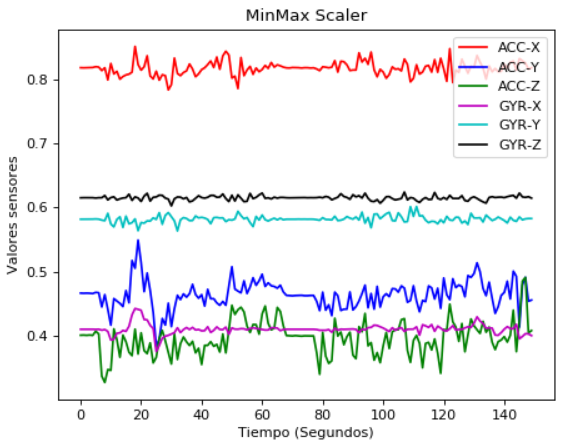
\includegraphics[width=\textwidth]{imagenes/Cap3/min_max}
            \caption{Min max Scaler}
            \label{fig:min_max}
        \end{subfigure}       
        \begin{subfigure}[h]{0.45\textwidth} 
            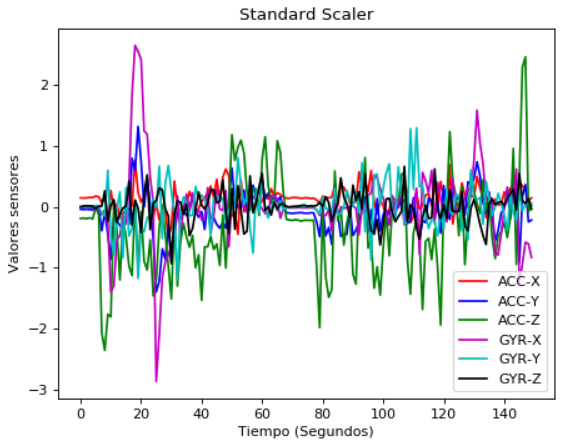
\includegraphics[width=\textwidth]{imagenes/Cap3/standard}
            \caption{Standard Scaler}
            \label{fig:standard}
        \end{subfigure}
        
        \begin{subfigure}[h]{0.45\textwidth} 
            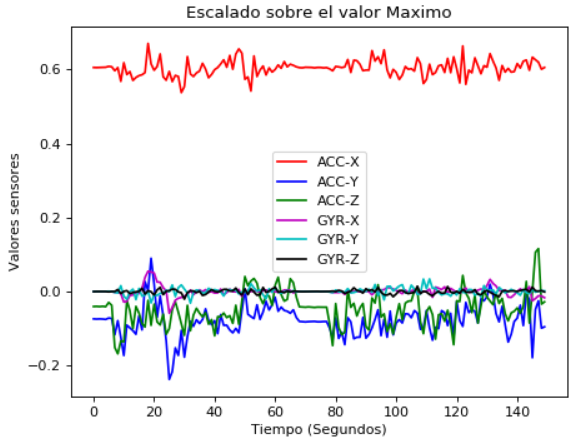
\includegraphics[width=\textwidth]{imagenes/Cap3/max}
            \caption{Max Scaler}
            \label{fig:max}
        \end{subfigure}       
        \begin{subfigure}[h]{0.45\textwidth} 
            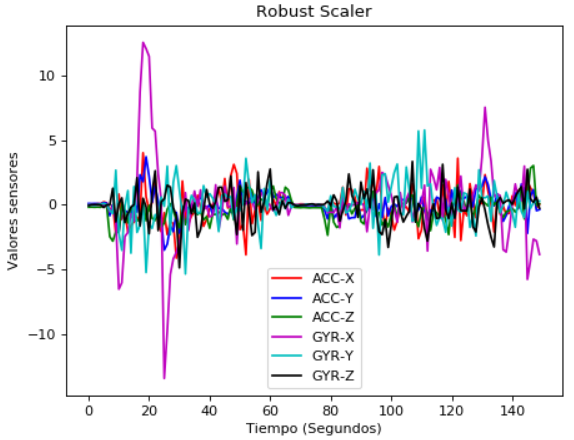
\includegraphics[width=\textwidth]{imagenes/Cap3/robust}
            \caption{Robust Scaler}
            \label{fig:robust}
        \end{subfigure}
        \caption{Gr\'{a}fica resultante de aplicar diferentes tipos de normalizaciones a un conjunto de datos.}
        
		\label{fig:nor_nor}
    \end{figure}

\section{Resumen del cap\'{i}tulo}

En este cap\'{i}tulo se ha descrito la forma en la que se realiz\'{o} la captura de datos de conducci\'{o}n, el an\'{a}lisis del conjunto de datos mediante t\'{e}cnicas estad\'{i}sticas y visuales y finalmente la elecci\'{o}n de un m\'{e}todo de normalizaci\'{o}n para comprimir los valores en un rango definido, para que de \'{e}sta manera estos valores sean una mejor entrada para el algoritmo de aprendizaje autom\'{a}tico que se aplicar\'{a} en el siguiente cap\'{i}tulo.
 